\addcontentsline{toc}{chapter}{Analiza i badania rynku}
Analiza biznesowa jest nieodłącznym elementem procesu planowania i podejmowania decyzji, które umożliwiającym lepsze zrozumienie kontekstu strategicznego, w jakim realizowany jest projekty. Polega ona na przygotowaniu zestawu zadań i technik, które stanowią łącznik między interesariuszami mając na celu zrozumienie w jaki sposób organizacje funkcjonują w dążeniu do osiągnięcia swoich celów. Ponadto, analiza biznesowa definiuje możliwości, których organizacja potrzebuje, aby skutecznie dostarczać produkty i usługi zewnętrznym interesariuszom \cite{businessanalysis}.

\section*{Analiza konkurencyjnych rozwiązań}
\addcontentsline{toc}{section}{Analiza konkurencyjnych rozwiązań}

Na rynku znajduje się wiele narzędzi do organizacji czasu, ale \textbf{kalendarz Google} (Rysunek \ref{fig:googleCalendar}) pozostaje niekwestionowanym liderem. Jest to profesjonalne i przede wszystkim darmowe, domyślne narzędzie na większości urządzeń z systemem Android.
Według raportu stworzonego przez zespół pracujący dla DataReportal, w Polsce na rok 2023, aż 87\% użytkowników posiada
telefon właśnie z tym systemem \cite{datareportal}. Aplikacja ta stanowi nieodłączny element funkcjonowania firm, zwłaszcza tych początkujących,
ale nie tylko. Ułatwia harmonogramowanie spotkań, śledzenie projektów i pozwala na zachowanie kontroli nad terminami.
Dużym atutem kalendarza Google jest rozdzielenie zadań i wydarzeń na osobne elementy.

Jest to narzędzie umożliwiające precyzyjne określenie wszelkich informacji odnośnie danego wydarzenia. Nie da się kwestionować, że możliwości jakie daje nam aplikacja są niepotrzebne, jednakże z punktu widzenia użytkownika końcowego ZodiaCal funkcje takie jak lokalizacja wydarzenia, link do rozmowy wideo czy określanie trwania każdego wydarzenia od do jest zbędne. W ZodiaCal istotne jest sprawne dodawanie wydarzeń do kalendarza, bez konieczności przeglądania dodatkowych opcji.

\newpage

Aplikacja \textbf{135 To Do List} (Rys. \ref{fig:ToDoList}), poprzez swój estetyczny i prosty interfejs ułatwia użytkownikom ustalanie priorytetów zadań na konkretny dzień.
Posiada możliwość zmiany kolejności wpisanych już wcześniej zadań oraz widok całego miesiąca.
Niestety nie ma opcji dodawania cyklicznych wydarzeń. ZodiaCal przyświeca niemalże ta sama minimalistyczna idea tworzenia interfejsu, jednak wprowadza rozbudowane funkcje, takie jak codzienny horoskop i osobisty dziennik pielęgnacji.

\begin{figure}
	\begin{minipage}{0.4\textwidth}
		\centering
		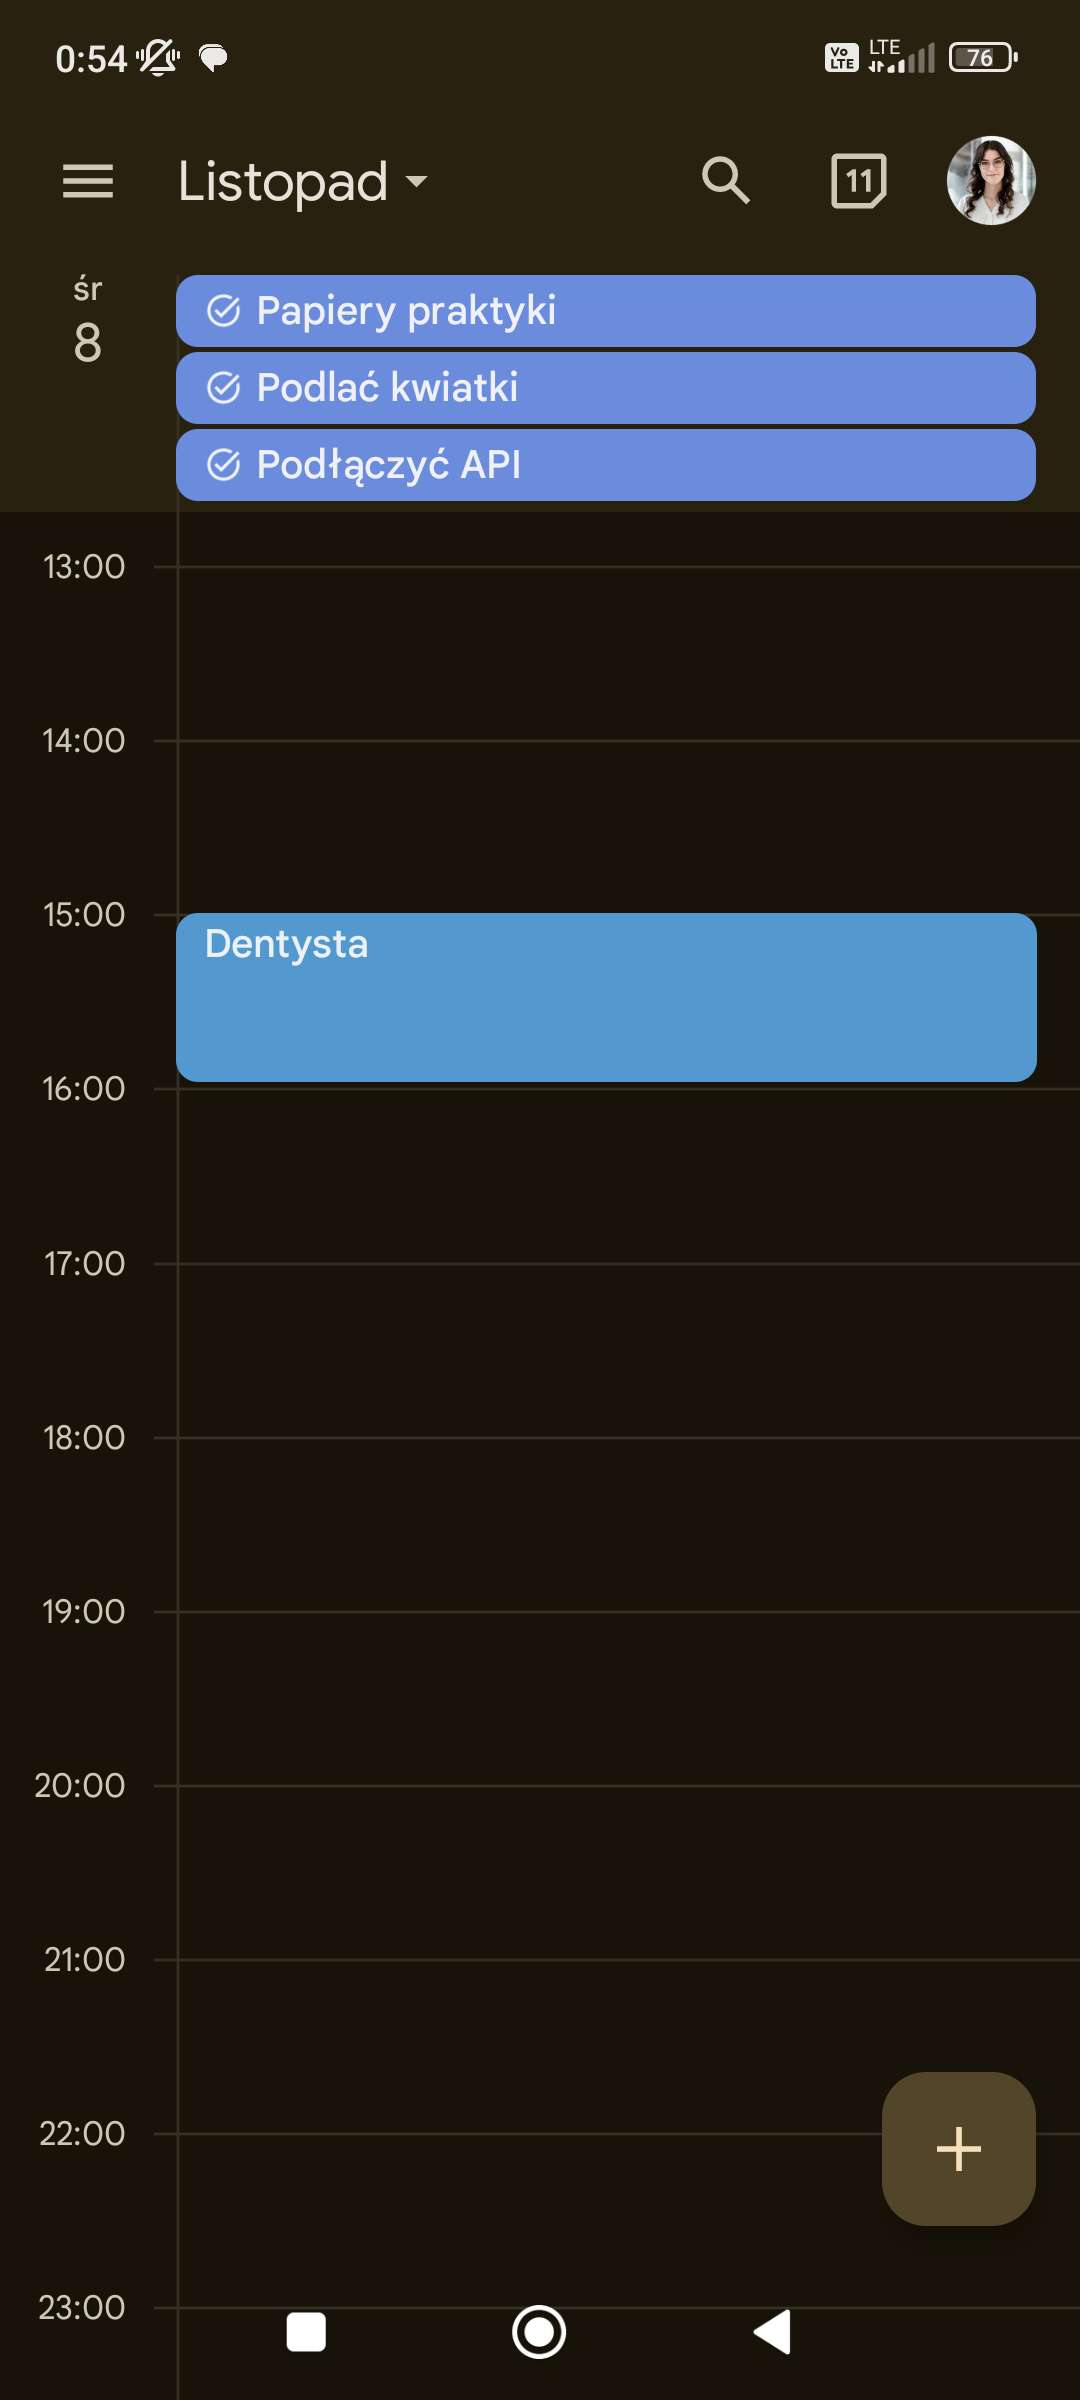
\includegraphics[height=10cm, keepaspectratio]{images/analiza/googleCalendar}
		\caption{Widok konkretnego dnia w kalendarzu Google}
		\label{fig:googleCalendar}
	\end{minipage}
	\hfill
	\begin{minipage}{0.4\textwidth}
		\centering
		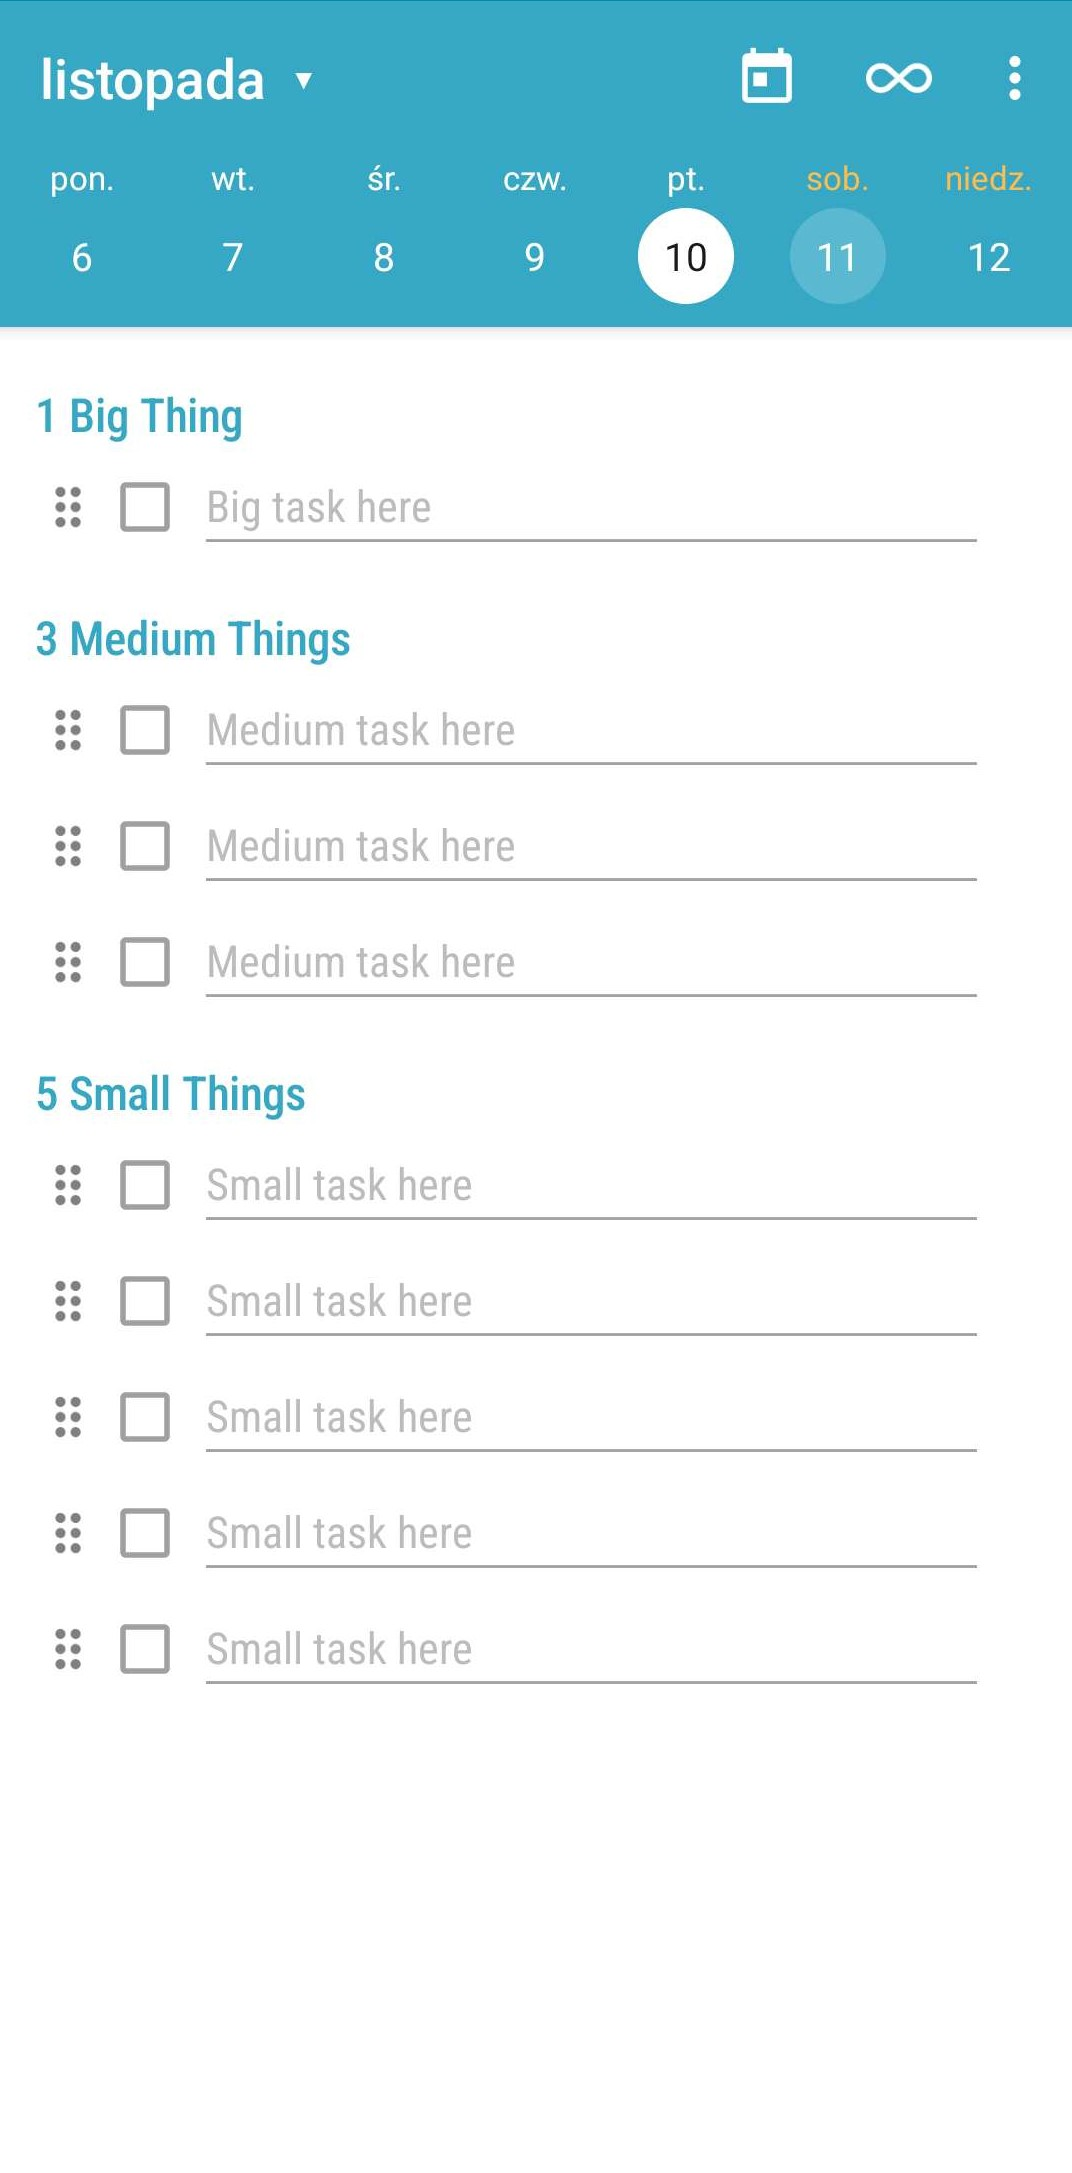
\includegraphics[height=10cm, keepaspectratio]{images/analiza/135ToDoList}
		\caption{Ekran główny aplikacji 135 To Do List}
		\label{fig:ToDoList}
	\end{minipage}
\end{figure}

Na rynku znajduje się wiele aplikacji oferujących dostęp do dziennych horoskopów. Są to głównie aplikacje dla silnie zaangażowanych w tym temacie użytkowników. \textbf{Daily Horoscope} (Rys. \ref{fig:dailyHoroscope}) oferuje wiele ciekawych rozwiązań takich jak funkcja przydzielania znaku zodiaku z podanej daty urodzenia. Niestety, aby otrzymać informację o znaku zodiaku użytkownik musi podać pełną datę urodzenia wraz z rokiem, w ZodiaCal wystarczy podać jedynie dzień i miesiąc. W dobie masowych wycieków danych, użytkownicy są szczególnie wyczuleni na podawanie swoich osobistych danych do różnego typu aplikacji. Dodatkowo Daily Horoscope koncentruje się nie tylko na astrologii zachodniej, ale również wschodniej. Zrozumiały jest fakt, że aplikacja o konkretnej tematyce będzie oferowała wiele rozbudowanych funkcji, jednak w ZodiaCal horoskop jest jedynie dodatkiem.


\textbf{FeelingMySkin} (Rys. \ref{fig:feelingMySkin}) to bardzo rozbudowane narzędzie do precyzyjnego określenia pielęgnacji cery i nie tylko.
Korzystając z niej użytkownik może układać plany pielęgnacyjne z wykorzystaniem konkretnych produktów,
których używa na co dzień, monitorować zmiany skórne, czy chociażby śledzić daty przydatności produktów.
To z pewnością przydatna aplikacja, jednakże wymaga czasu, aby opanować wszystkie możliwe funkcje.
Interfejs strony głównej jest bardzo przeładowany informacjami, co utrudnia korzystanie z aplikacji w sposób efektywny.

\begin{figure}[t]
  \begin{minipage}{0.4\textwidth}
    \centering
    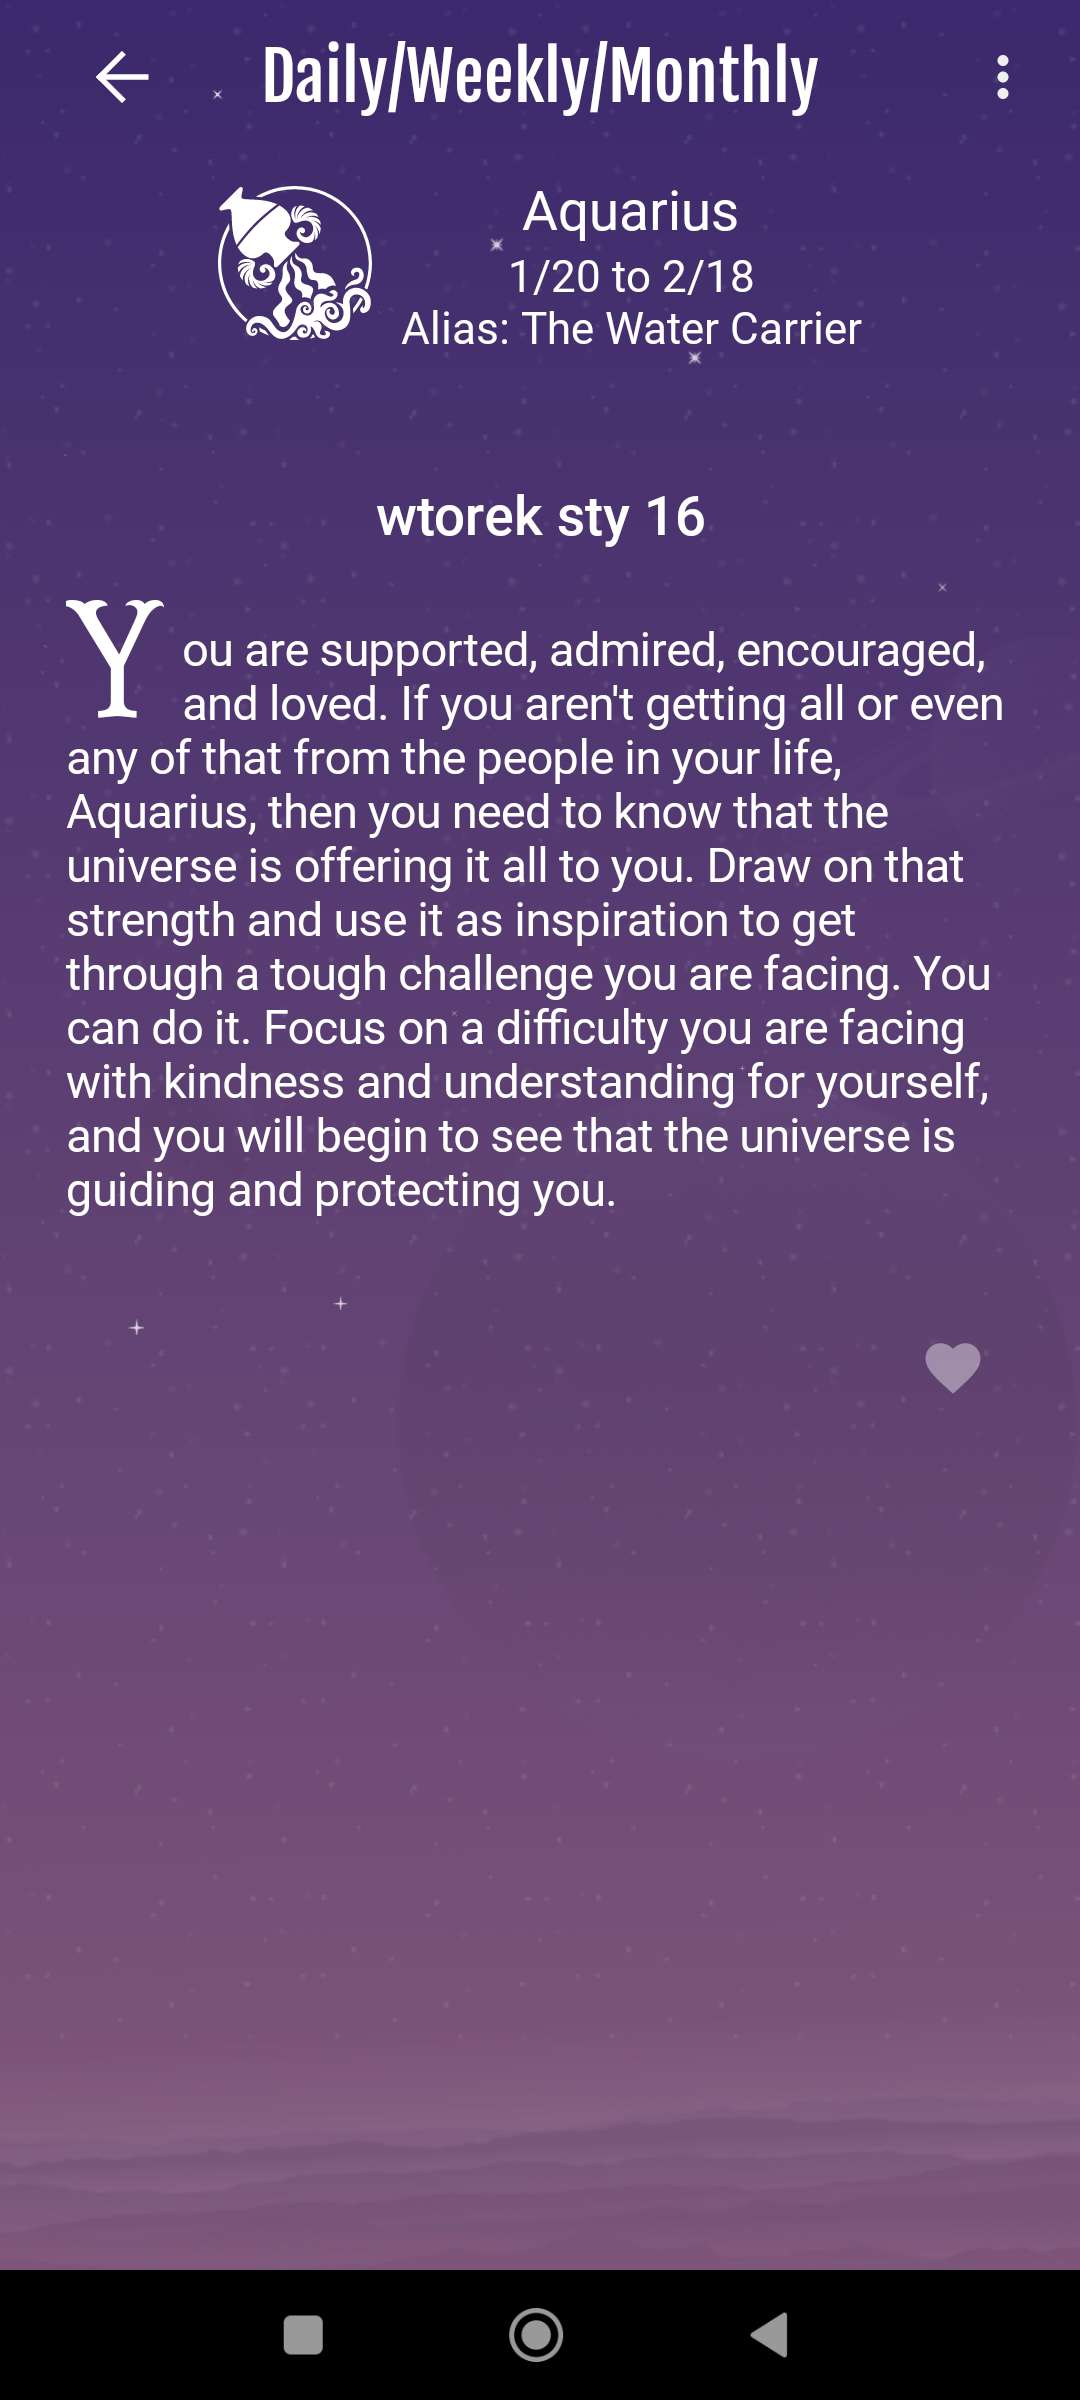
\includegraphics[height=10cm, keepaspectratio]{images/analiza/dailyHoroscope}
    \caption{Widok horoskopu dziennego w aplikacji Daily Horoscope}
    \label{fig:dailyHoroscope}
  \end{minipage}
  \hfill
  \begin{minipage}{0.4\textwidth}
    \centering
    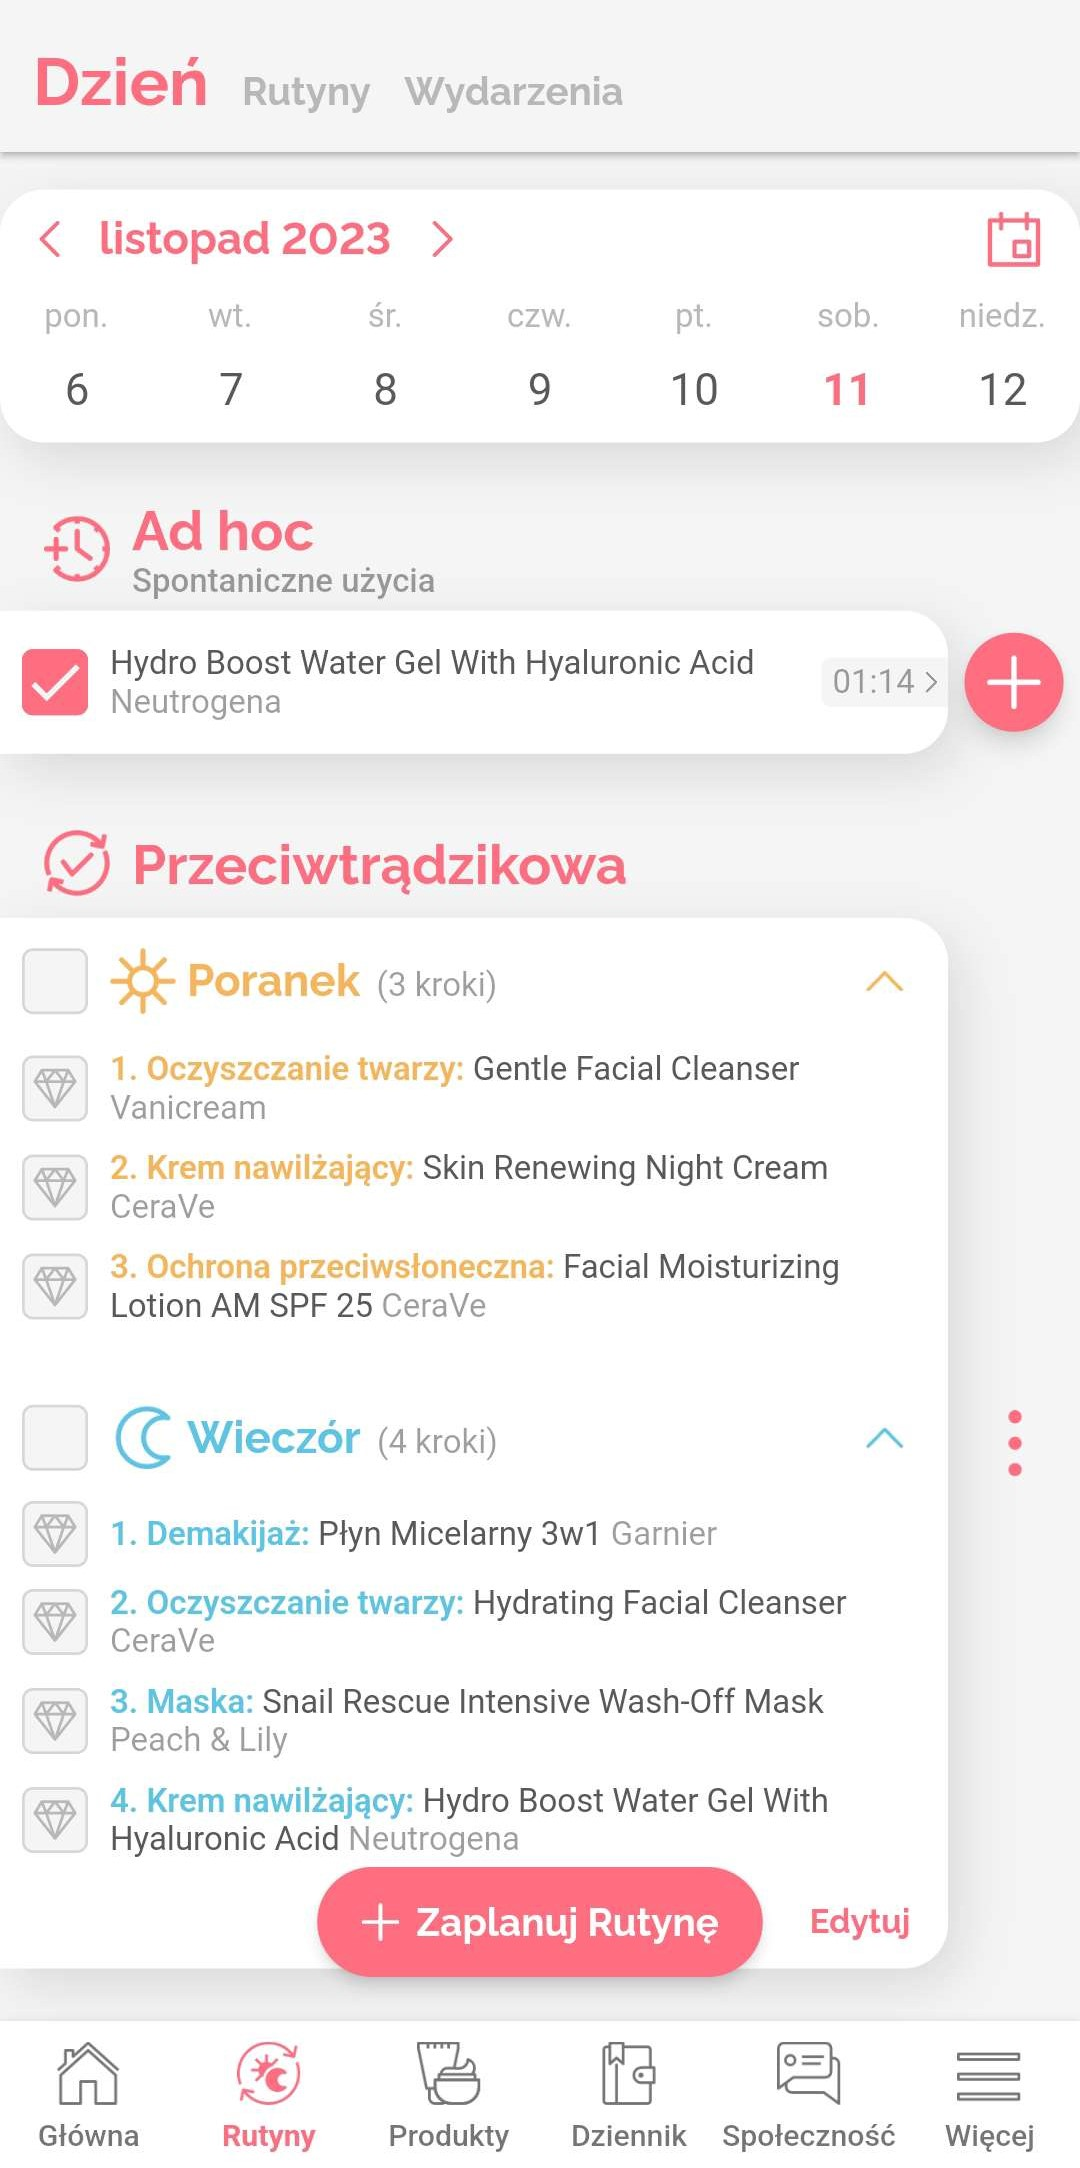
\includegraphics[height=10cm, keepaspectratio]{images/analiza/feelingMySkin}
    \caption{Widok codziennej rutyny w aplikacji FeelingMySkin}
    \label{fig:feelingMySkin}
  \end{minipage}
\end{figure}

ZodiaCal to hybryda wszystkich wymienionych aplikacji.
To minimalistyczne narzędzie służące do wielu celów, ale w podstawowym zakresie. Próbuje połączyć najlepsze cechy różnych istniejących aplikacji,
oferując minimalistyczny interfejs do zarządzania czasem, zadaniami i nie tylko. Chociaż nie zawiera wszystkich zaawansowanych funkcji dostępnych w innych aplikacjach, dąży do dostarczenia użytkownikom wyważonego narzędzia do pracy.

\section*{Analiza SWOT}
\addcontentsline{toc}{section}{Analiza SWOT}
\phantom{th}
Analiza SWOT to termin powstały od pierwszych liter poszczególnych słów w języku angielskim,
czyli Strengths - siły, Weaknesses - słabości, Opportunities - szanse oraz Threats - zagrożenia.
Jest to metoda analizy rynku, która cieszy się popularnością wśród współczesnych przedsiębiorców.
Takie podejściu do projektu pozwala na lepsze zrozumienie wpływów istniejących już warunków na przyszłość,
szybkie określenie planów strategicznych oraz ułatwia podejmowania decyzji.
Cieszy się popularnością ze względu na prostotę oraz skuteczność działania \cite{businessanalysis}.

\subsubsection*{\textbf{Mocne strony (Strengths):}}
Czynniki aplikacji, które podnoszą jej przewagę konkurencyjną. W tej chwili rynek rozdziela kalendarz osobisty i dzienniczek pielęgnacji na dwie różne aplikację,
co prowadzi do tego, że użytkownik nie tylko musi uzupełniać pola w dwóch różnych miejscach,
uczyć się dwóch różnych interfejsów, ale również przekazywać swoje dane do dwóch różnych serwisów.
Interfejsy wymienionych aplikacji posiadają wiele funkcji do precyzyjnego określania zadań
czy pielęgnacji przez co opanowanie ich zajmuje więcej czasu i wysiłku użytkownika,
niż gdyby posiadały jedynie podstawowe funkcje w tym zakresie.
Aplikacja została stworzona z myślą o wielu platformach dzięki czemu może dotrzeć do szerszej grupy odbiorców.
Opcja, której nie spotkamy w żadnym innym kalendarzu to możliwość sprawdzenia codziennego horoskopu dostosowanego do znaku zodiaku użytkownika.
Dodatkowo, jeśli użytkownik nie wie w jaki sposób określić swój znak zodiaku, aplikacji zrobi to za niego, wystarczy podać dzień i miesiąc urodzenia.

\subsubsection*{\textbf{Słabe strony (Weaknesses):}}
Czynniki aplikacji, które osłabiają jej pozycję. Prostota jest jednocześnie zaletą i wadą. Wadą, ponieważ może nie spełniać oczekiwań zaawansowanych użytkowników,
którym może brakować pewnych funkcji. Brak bazy danych produktów to kolejna słabość projektu.
W aplikacji nie ma możliwości wybrania z bazy danych kosmetyków, których użytkownik używa podczas pielęgnacji jak to mam miejsce w FeelingMySkin.
Opcja ta jest nie dostępna, ponieważ wiązałaby się z podpięciem do przekraczającej wielkościami bazy danych
oraz nieustanne aktualizowanie jej za każdym nowym wprowadzonym produktem na rynek.
Innym negatywnym aspektem jest fakt, iż obecnie rynek przepełniony jest aplikacjami o podobnym charakterze. W związku z tym konieczne może być przeprowadzenie skutecznej kampanii reklamowej, aby wyróżnić aplikację wśród konkurencji.

\subsubsection*{\textbf{Szanse (Opportunities):}}
Czynniki zewnętrzne, które mają pozytywny wpływ na obecną sytuację na rynku. Ostatnio obserwuje się rosnące zainteresowanie świadomą pielęgnacją skóry, co przekłada się na wzrost zapotrzebowania na aplikacje ułatwiające planowanie pielęgnacji, czy monitorowanie stanów skóry.


\subsubsection*{\textbf{Zagrożenia (Threats):}}
Czynniki zewnętrzne, które mogą negatywnie wpłynąć na aplikację. Największym wyzwaniem jest zagwarantowanie prywatności i bezpieczeństwa danych. Konieczne jest zapewnienie wysokiego poziomu ochrony danych użytkowników, zwłaszcza w obszarze związanym z informacjami o pielęgnacji skóry, które uważane są za dane wrażliwe. Następnym wadliwym punktem są zmiany w regulacjach dotyczących prywatności w różnych państwach.
Zmiany przepisów dotyczących ochrony danych osobowych mogą wymagać dostosowania polityki prywatności aplikacji,
w związku z tym, istotne jest, aby systematycznie monitorować ewentualne zmiany w przepisach.
